\section{Experiments}\label{experiments}

In this section, we demonstrate the effectiveness of the algorithm presented in Section~\ref{algorithm} in the context of movement primitive learning for optimal striking motions. We consider two hitting tasks: putting in golf and ball-hitting in table tennis. In each task trajectories and the extracted movement primitives are assigned in joint space, one for each joint of the robot. 

We assume that the reference trajectories are \emph{feasible}, i.e. that it is possible to follow them arbitrarily well. If this assumption does not hold, then one can enforce feasibility by redesigning the basis functions $\basis(t)$ of the DMPs so as to filter out the nonsmooth parts of the trajectory adequately.

\subsection{Putting}

Putting is a simple and natural domain for testing ILC algorithms because it allows a robot to apply ILC to control few degrees of freedom (typically the end joint) while having the dynamics of the other joints act as disturbances. This kind of learning in underactuated dynamical systems can act as a scalable interface to more complex hitting tasks in the full-joint space of the robot. By learning a causal map of the robot (i.e. a graphical model) one can iteratively construct increasingly sophisticated controllers that is cognizant of the causal relationships between the joints. Here we provide only a simple example of such \emph{scalable} learning. 

We first provide a simulation of a two-joint robot that has a golf stick attached to the end-effector at the second joint. Accounting for the simulated friction between the golf ball and the hole, we come up with a cycloid reference trajectory that intercepts the ball with a desired velocity of 1 m/s at the 95 percent part of the trajectory before decelerating significantly and coming to a halt. We can easily capture this effect with a DMP.

The initial trial (iteration one) is shown in Figure X. Here we can see how the first joint of the robot prevents the second joint from following the trajectory precisely. The following iterations show how ILC compensates for such an effect and in the last iteration the ball goes straight into the hole without any significant deviation from the linear path between them. We compare the approach with \emph{REPS} and \emph{PI$^{2}$} in Figure X by plotting the RMS-error of the iterations with each algorithm. Notice that these stochastic approaches take much longer to converge.

\subsection{Table Tennis}

% hitting is not at the end of the trajectory

As a second and more complex task, we consider table tennis where we are interested in generating and executing accurate ball-hitting motions. For the robotic table tennis task we are using a seven degree of freedom (DoF) Barrett WAM arm capable of high speeds up to X rad/sec. A standard size racket (16 cm diameter) is mounted on the end-effector of the arm as can be seen in Figure X. A vision system consisting of four cameras hanging from the ceiling around each corner of the table is used for tracking the ball \cite{Lampert12}. The orange ball is tracked  visually with a sampling rate of 60 Hz and filtered with an extended Kalman filter that accounts for some of the bouncing behaviour of the ball and air drag effects. The table and the tennis balls are in accordance with the International Table Tennis Federation (ITTF) rules.

A ball launcher (see Figure X) is available to throw balls accurately to a fixed position in cartesian space to the forehand of the robot. The incoming ball arrives with low-variability in desired positions and higher-variability in ball velocities. The whole area to be covered amounts to about 1 m$^2$ circular region in front of the initial forehand gesture of the robot, see Figure X. This allows us to avoid the singularities of the robot. Any ball that appears outside of this circular \emph{feasible} region will not be hit.

When the visual system provides a trajectory of the robot that coincides with the feasible region in cartesian space, the system has to come up with a trajectory that specifices how, where and when to intersect the incoming ball trajectory. Desired cartesian position, velocity and orientation of the racket translates in joint space to the specification of 14 parameters: 7 joint angles and 7 joint velocities of the robot arm. Along with the desired hitting time (or the time until impact), these 15 parameters are used to train 7 joint space DMPs that corresponds to the desired reference trajectory in cartesian space. These movement primitives are synchronized with the same phase \eqref{phase}.

% maybe work on this kinesthetic teach-in paragraph more
In order to generate feasible reference trajectories that account for the variation in incoming ball position and velocity, we used kinesthetic teach-in on the robot to generate successful hitting motions, i.e. those that can hit the ball to the opponent's court. Using the successful examples we trained a probabilistic model $p(\weights|\state_b)$ given ball positions $\state_b$ using weighted regression. Weighting can be put in various ways and we opted for a weighting which put a higher reward on the fast strikes that landed on the edges. The generated DMPs of the model are guaranteed to be safe because these movements lie within the convex combination of demonstrations. 
% Katharina - Hence, the system will not encounter joint limits or hit the table.

% scale dmps if provided with better estimation data of ball position and velocity. dmps as opposed to control inputs or even trajectories can be easily extended to allow for this. 

% From Katharina's paper:
%the position, velocity and orientation of the racket can be computed analytically based on the state of the system and the target on the opponents court.
%These task space parameters can also be converted into joint space parameters using inverse kinematics

\begin{figure}
\center
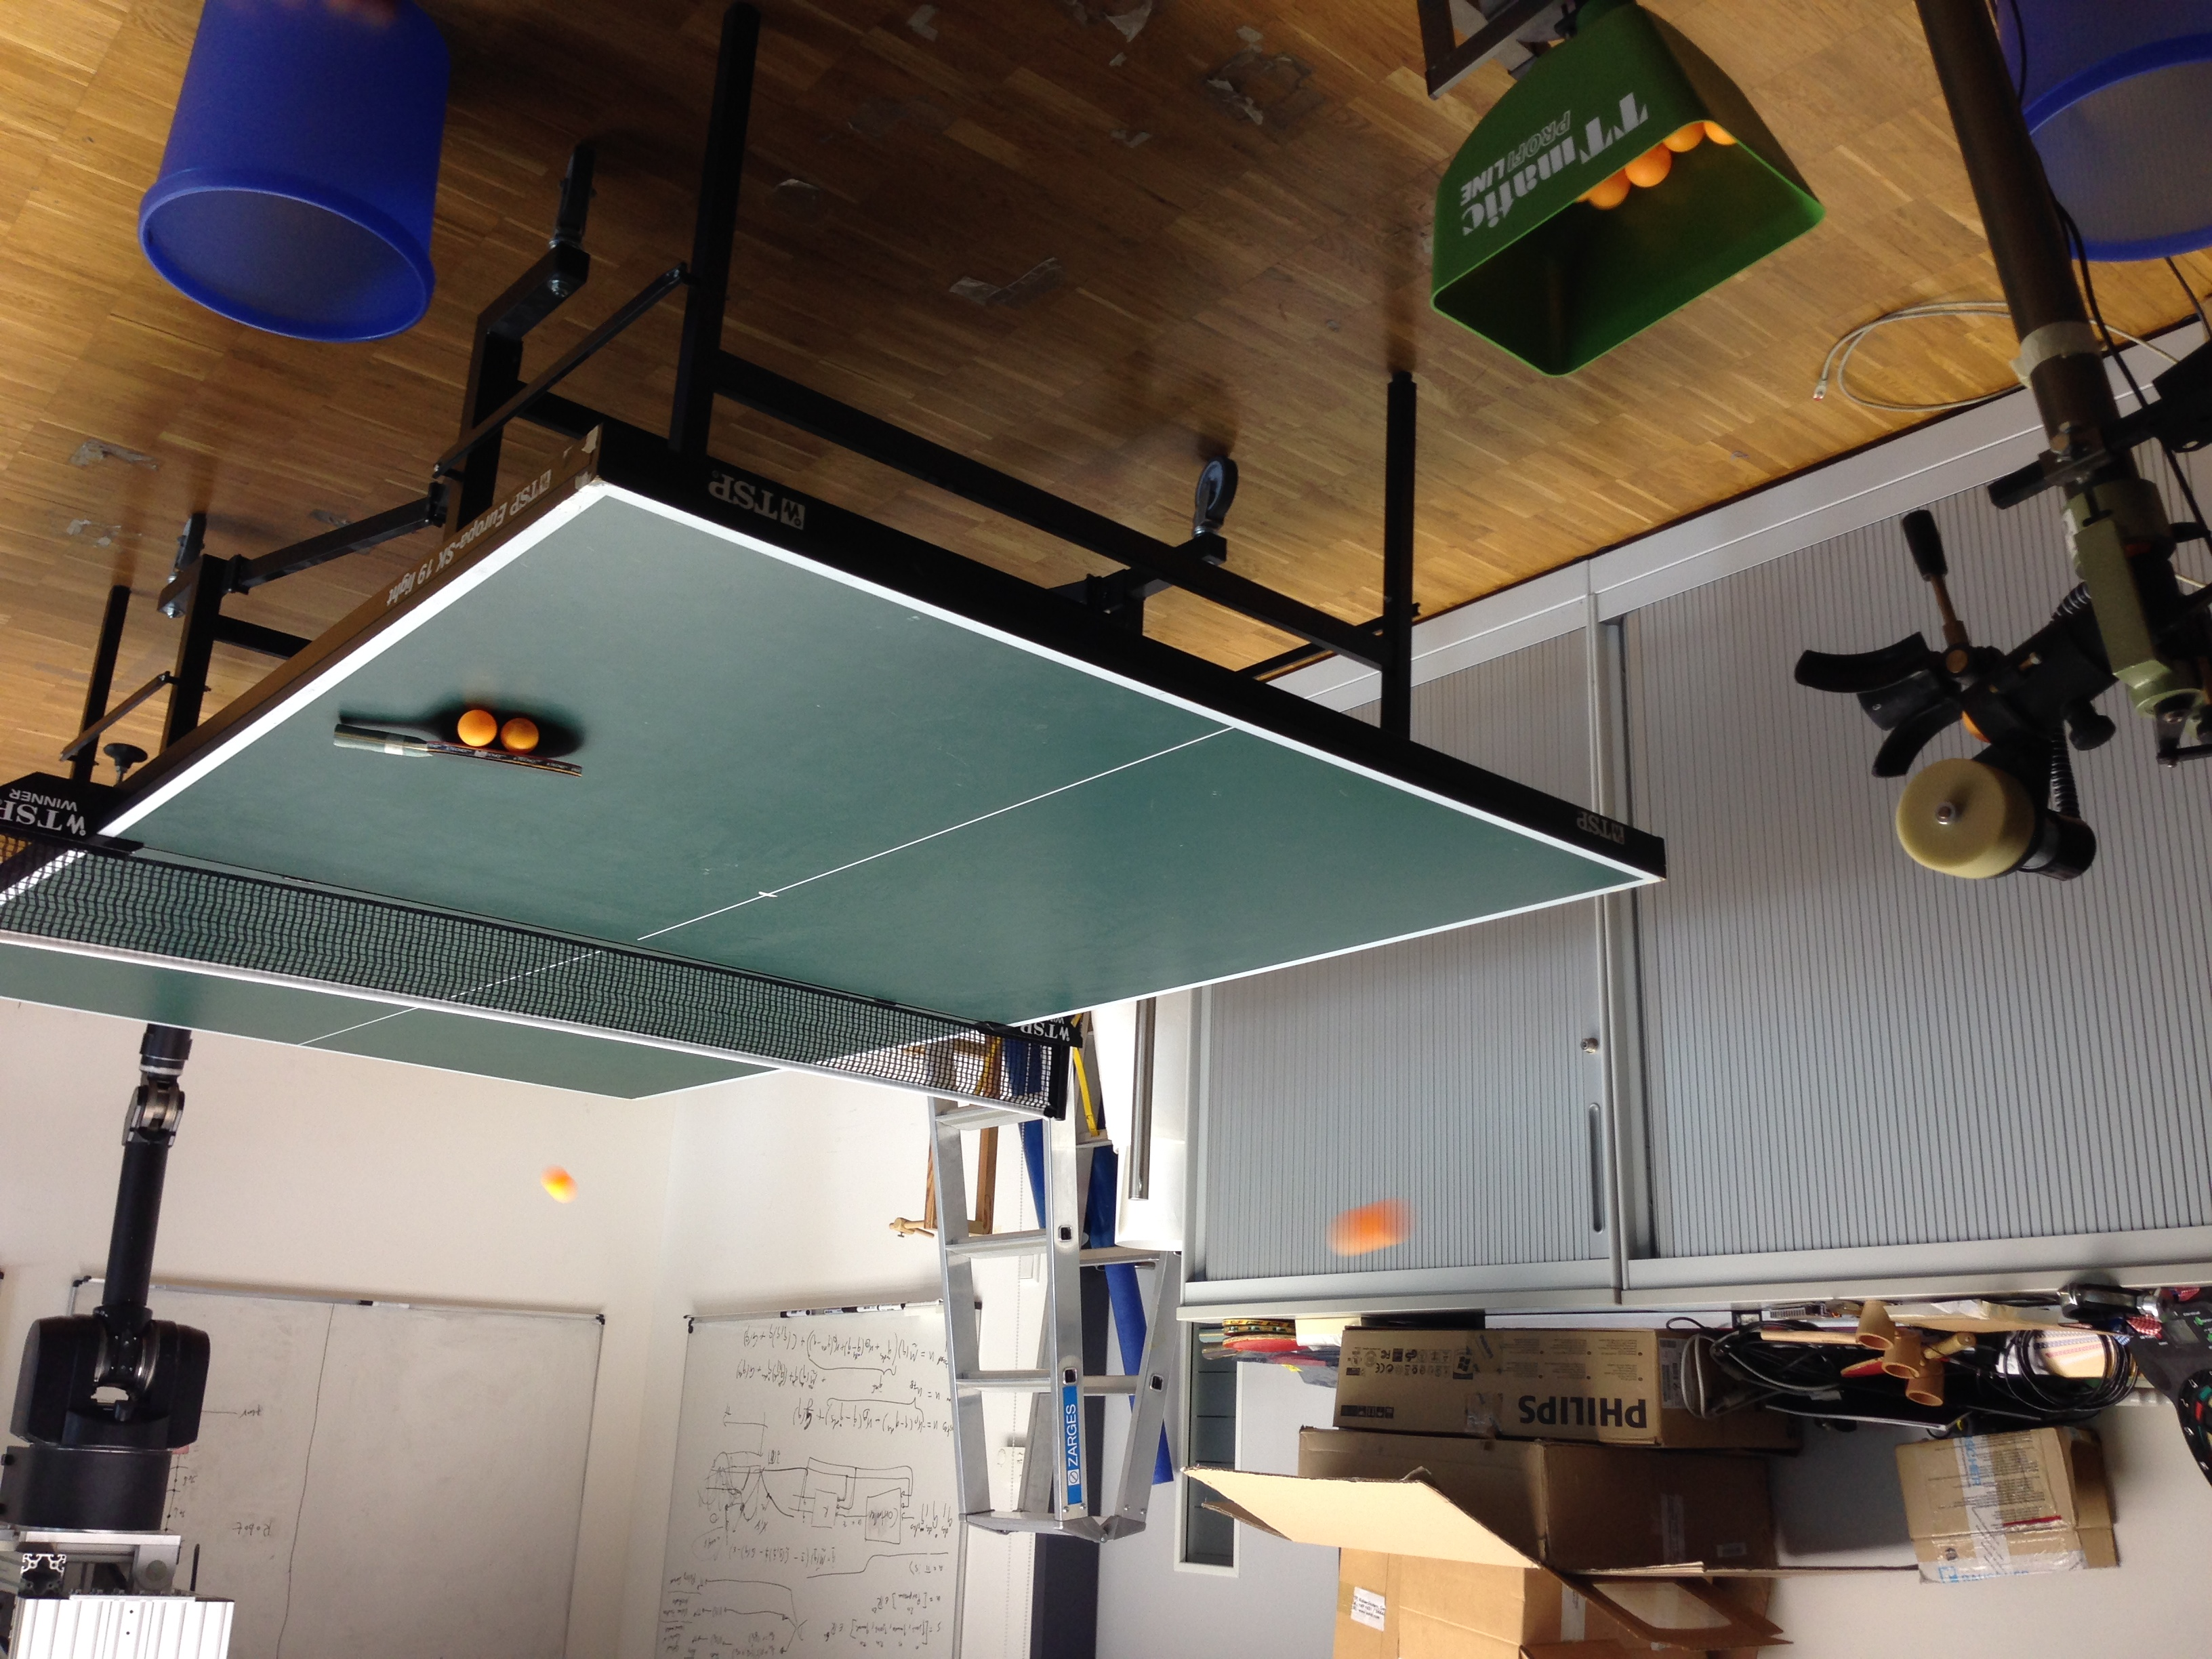
\includegraphics[scale=0.05, angle= 180]{ballgun.jpg}			
\caption{Robotic table tennis setup with the ballgun throwing balls to the robot}
\label{barrettArm}
\end{figure}

The attached video shows the improvement achieved after using our algorithm $\alg$. In order to apply our method to a given reference trajectory, we use the mode of the empirical distribution $p(\weights,\state_b) = p(\weights|\state_b)p(\state_b)$ as our initial movement primitive. The convergence of the trajectories over the iteration domain are shown in cartesian space in Figure X. Some examples of the generated trajectories for the joints 5, 6 and 7 are given in Figure X. Comparisons to episodic-RL algorithms \emph{REPS} and \emph{PI$^{2}$} in Figure X illustrate the benefits of our approach, especially the faster convergence and increased accuracy of the proposed method.